\documentclass[tikz,border=10pt]{standalone}
\usepackage{tikz}
\usepackage{amsmath,amssymb}
\usetikzlibrary{positioning, arrows.meta, shapes.geometric, fit, backgrounds, calc, decorations.pathreplacing}

\begin{document}

% ★★★ 调整这个值来控制下半部分的左移程度 ★★★
\newcommand{\lowershift}{-.7}  % 负值=左移,正值=右移

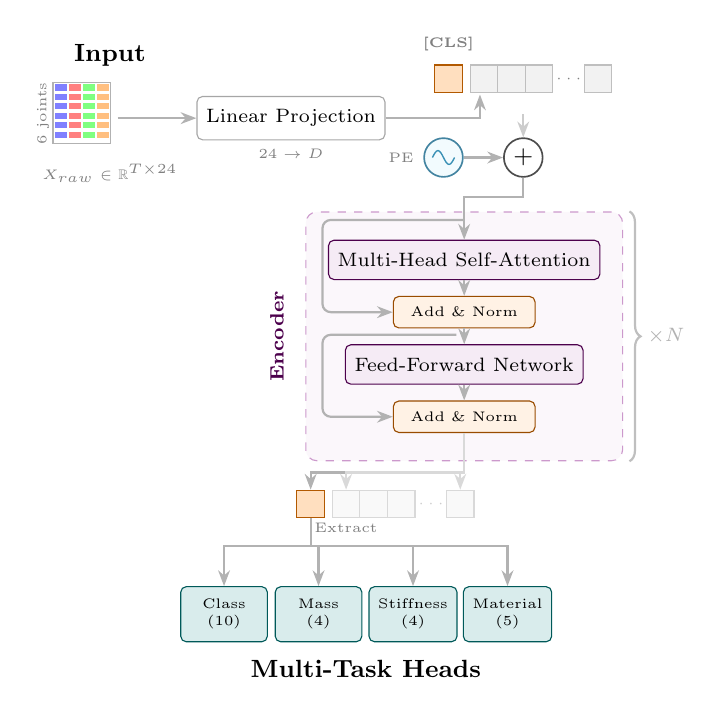
\begin{tikzpicture}[
    node distance=0.6cm,
    >={Stealth[length=2mm]},
    % 样式定义
    block/.style={draw=gray!70, fill=white, rounded corners=2pt,
                  minimum width=2.2cm, minimum height=0.55cm, font=\scriptsize},
    transblock/.style={draw=violet!60!black, fill=violet!8, rounded corners=2pt,
                       minimum width=2.4cm, minimum height=0.5cm, font=\scriptsize},
    clstoken/.style={draw=orange!70!black, fill=orange!25, 
                     minimum width=0.35cm, minimum height=0.35cm, font=\tiny},
    seqtoken/.style={draw=gray!50, fill=gray!10, 
                     minimum width=0.35cm, minimum height=0.35cm, font=\tiny},
    head/.style={draw=teal!70!black, fill=teal!15, rounded corners=2pt,
                 minimum width=1.1cm, minimum height=0.7cm, font=\tiny, align=center},
    circleop/.style={circle, draw=black!70, fill=white, 
                     minimum size=14pt, font=\small, inner sep=0pt, line width=0.6pt},
    arrow/.style={->, thick, gray!60},
    annot/.style={font=\tiny, gray},
    title/.style={font=\bfseries\small}
]

% ========== 1. 输入层 ==========
\node[title] at (-3.5, 0.8) {Input};

% 6个关节 × 4信号 的矩阵表示
\begin{scope}[shift={(-3.5, 0)}]
    % 画 6 行(关节)× 4 列(信号)的小方块矩阵
    \foreach \j in {0,1,2,3,4,5} {
        % Position (蓝)
        \fill[blue!50] (-0.7, 0.35-\j*0.12) rectangle (-0.55, 0.43-\j*0.12);
        % Current (红)
        \fill[red!50] (-0.52, 0.35-\j*0.12) rectangle (-0.37, 0.43-\j*0.12);
        % Velocity (绿)
        \fill[green!50] (-0.34, 0.35-\j*0.12) rectangle (-0.19, 0.43-\j*0.12);
        % Load (橙)
        \fill[orange!50] (-0.16, 0.35-\j*0.12) rectangle (-0.01, 0.43-\j*0.12);
    }
    % 外框
    \draw[gray!60, line width=0.5pt] (-0.72, -0.32) rectangle (0.01, 0.45);
    % 标注
    \node[font=\tiny, gray, rotate=90] at (-0.85, 0.06) {6 joints};
\end{scope}

\node[annot, align=center] at (-3.5, -0.7) {$X_{raw} \in \mathbb{R}^{T \times 24}$};

% ========== 2. 线性投影 ==========
\node[block] (proj) at (-1.2, 0) {Linear Projection};
\node[annot] at (-1.2, -0.45) {$24 \to D$};

\draw[arrow] (-3.4, 0) -- (proj.west);

% ========== 3. Token 序列 + CLS ==========
% CLS token
\node[clstoken] (cls) at (0.8, 0.5) {};
\node[annot, above=0.05cm of cls] {\textbf{[CLS]}};

% 序列 tokens
\node[seqtoken] (t1) at (1.25, 0.5) {};
\node[seqtoken] (t2) at (1.6, 0.5) {};
\node[seqtoken] (t3) at (1.95, 0.5) {};
\node[annot] at (2.35, 0.5) {$\cdots$};
\node[seqtoken] (tn) at (2.7, 0.5) {};

% 折线箭头:proj -> 下方 -> tokens 下方 -> 向上连接
\draw[arrow] (proj.east) -- ++(0.3, 0) |- (1.2, 0.0) -- (1.2, 0.3);

% ========== 4. 位置编码 ==========
\node[circleop] (pe_plus) at (1.75, -0.5) {+};

% PE 圆圈带正弦波
\node[circle, draw=cyan!60!black, fill=cyan!5, minimum size=14pt, 
      left=0.5cm of pe_plus, line width=0.6pt] (pe_circle) {};
\draw[cyan!70!black, line width=0.5pt] 
    ([xshift=-4pt]pe_circle.center) 
    sin ++(2pt, 2.5pt) cos ++(2pt, -2.5pt) sin ++(2pt, -2.5pt) cos ++(2pt, 2.5pt);
\node[annot, left=0.0001cm of pe_circle] {PE};

\draw[arrow] (pe_circle.east) -- (pe_plus.west);
\draw[arrow, gray!40] (1.75, 0.05) -- (pe_plus.north);

% ========== 5. Transformer Encoder ==========
% Add & Norm 样式
\tikzset{addnorm/.style={draw=orange!60!black, fill=orange!10, rounded corners=2pt,
                         minimum width=1.8cm, minimum height=0.4cm, font=\tiny}}

\node[transblock] (msa) at (\lowershift, -1.8) {Multi-Head Self-Attention};
\node[addnorm, below=0.2cm of msa] (an1) {Add \& Norm};
\node[transblock, below=0.2cm of an1] (ffn) {Feed-Forward Network};
\node[addnorm, below=0.2cm of ffn] (an2) {Add \& Norm};

% 残差连接 1: 绕过 MSA (从 north 上方连出)
\draw[arrow, rounded corners=3pt] 
    ($(msa.north)+(0, 0.25)$) -- ++(-1.8, 0) |- (an1.west);

% 残差连接 2: 绕过 FFN
\draw[arrow, rounded corners=3pt] 
    ($(an1.south)+(-0.1, -0.08)$) -- ++(-1.7, 0) |- (an2.west);

% Transformer 大框
\begin{scope}[on background layer]
    \node[draw=violet!40, fill=violet!3, dashed, rounded corners=4pt, 
          fit=(msa)(an2), inner sep=8pt, inner ysep=10pt] (trans_box) {};
\end{scope}

% Transformer Encoder 标签竖排在左边
\node[font=\scriptsize\bfseries, violet!60!black, rotate=90, anchor=south] 
    at ($(trans_box.west)+(-0.15,0)$) {Encoder};

% x N 标注
\draw[decorate, decoration={brace, amplitude=4pt, mirror}, thick, gray!50] 
    ($(trans_box.south east)+(0.08,0)$) -- ($(trans_box.north east)+(0.08,0)$)
    node[midway, right=0.1cm, font=\scriptsize\bfseries, gray!60] {$\times N$};

\draw[arrow] (pe_plus.south) |-(\lowershift,-1.0) --(msa.north);
\draw[arrow] (msa) -- (an1);
\draw[arrow] (an1) -- (ffn);
\draw[arrow] (ffn) -- (an2);

% ========== 6. 输出序列 ==========
% CLS token (高亮)
\node[clstoken] (cls_out) at (\lowershift-0.95, -4.9) {};
% 其他 tokens (淡化)
\node[seqtoken, fill=gray!5, draw=gray!30] (t1_out) at (\lowershift-0.5, -4.9) {};
\node[seqtoken, fill=gray!5, draw=gray!30] (t2_out) at (\lowershift-0.15, -4.9) {};
\node[seqtoken, fill=gray!5, draw=gray!30] (t3_out) at (\lowershift+0.2, -4.9) {};
\node[annot, gray!40] at (\lowershift+0.6, -4.9) {$\cdots$};
\node[seqtoken, fill=gray!5, draw=gray!30] (tn_out) at (\lowershift+0.95, -4.9) {};

\draw[arrow] (an2.south) -- ++(0, -0.5) -| (cls_out.north);
\draw[arrow, gray!30] (an2.south) -- ++(0, -0.5) -| (t1_out.north);
\draw[arrow, gray!30] (an2.south) -- ++(0, -0.5) -| (tn_out.north);

\node[annot] at (\lowershift-0.5, -5.2) {Extract};

% ========== 7. 多任务头 ==========
\node[head] (h_class) at (\lowershift-2.05, -6.3) {Class\\(10)};
\node[head] (h_mass) at (\lowershift-0.85, -6.3) {Mass\\(4)};
\node[head] (h_stiff) at (\lowershift+0.35, -6.3) {Stiffness\\(4)};
\node[head] (h_mat) at (\lowershift+1.55, -6.3) {Material\\(5)};

% 从 CLS 连接到各个 head
\draw[arrow] (cls_out.south) -- ++(0, -0.35) -| (h_class.north);
\draw[arrow] (cls_out.south) -- ++(0, -0.35) -| (h_mass.north);
\draw[arrow] (cls_out.south) -- ++(0, -0.35) -| (h_stiff.north);
\draw[arrow] (cls_out.south) -- ++(0, -0.35) -| (h_mat.north);

% 多任务头标签
\node[title] at (\lowershift-0.25, -7.0) {Multi-Task Heads};

\end{tikzpicture}

\end{document}
